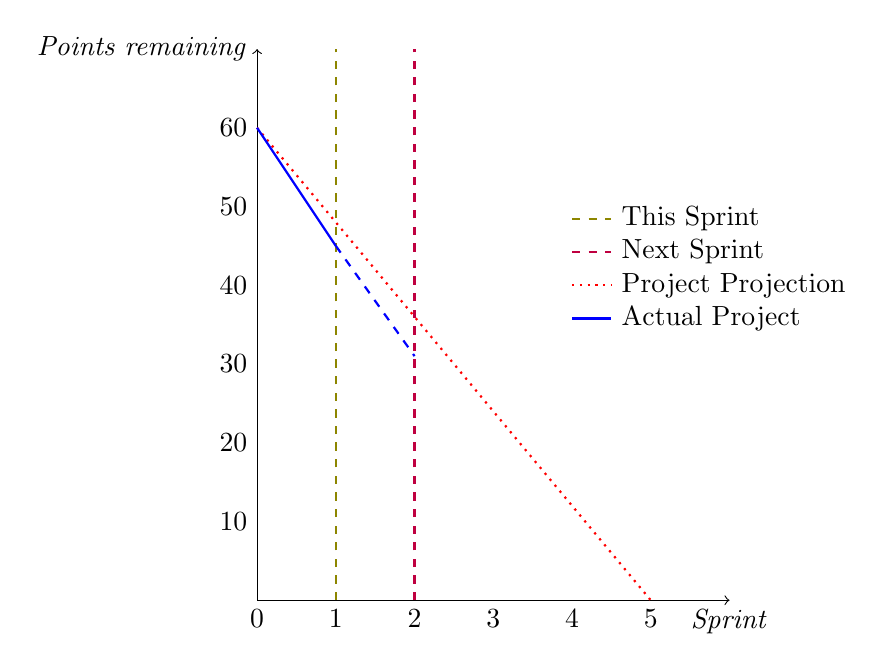
\begin{tikzpicture}

% horizontal axis
    \draw[->] (0,0) -- (6,0) node[anchor=north] {\emph{Sprint}};
% labels
    \draw   (0,0) node[anchor=north] {0}
            (1,0) node[anchor=north] {1}
            (2,0) node[anchor=north] {2}
            (3,0) node[anchor=north] {3}
            (4,0) node[anchor=north] {4}
            (5,0) node[anchor=north] {5};

% vertical axis
    \draw[->] (0,0) -- (0,7) node[anchor=east] {\emph{Points remaining}};
% labels
    \draw   (0,1) node[anchor=east] {10}
            (0,2) node[anchor=east] {20}
            (0,3) node[anchor=east] {30}
            (0,4) node[anchor=east] {40}
            (0,5) node[anchor=east] {50}
            (0,6) node[anchor=east] {60};

% current sprint 
    \draw[thick, dashed, olive] (1,0) -- (1,7);
% label
    % \draw (3,3.7.5) node[anchor=east] {\emph{This Sprint}};

% next sprint 
    \draw[thick, dashed, purple] (2,0) -- (2,7);
% label
    % \draw (4.4,6.5) node[anchor=east] {\emph{Next Sprint}};

% projected 
    \draw[thick, dotted, red] (0,6) -- (5,0);
% actual
    \draw[thick, blue] (0,6) -- (1,4.5);
% actual
    \draw[thick, dashed, blue] (1,4.5) -- (2,3.1);
    
\begin{scope}[shift={(4,4)}] 
    \draw[thick, dotted, red] (0,0) -- (0.5,0) 
        node[black, right]{Project Projection};
    \draw[thick, blue, yshift=\baselineskip * - 1] (0,0) -- (0.5,0)
        node[black, right]{Actual Project};
    \draw[thick, dashed, purple, yshift=\baselineskip] (0,0) -- (0.5,0)
        node[black, right]{Next Sprint};
    \draw[thick, dashed, olive, yshift=\baselineskip * 2] (0,0) -- (0.5,0)
        node[black, right]{This Sprint};
\end{scope}

\end{tikzpicture}
